\tikzset{every picture/.style={line width=0.75pt}} %set default line width to 0.75pt        
\begin{center}
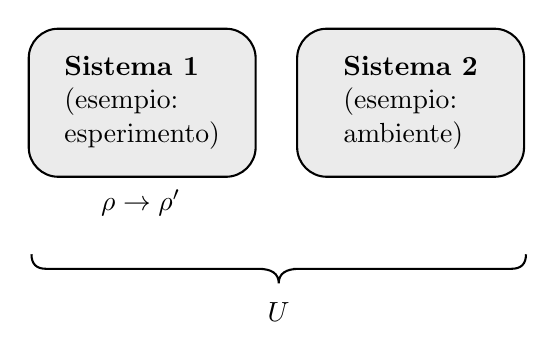
\begin{tikzpicture}[x=0.75pt,y=0.75pt,yscale=-1,xscale=1]
%uncomment if require: \path (0,300); %set diagram left start at 0, and has height of 300

%Rounded Rect [id:dp6009925516212442] 
\draw  [fill={rgb, 255:red, 194; green, 194; blue, 194 }  ,fill opacity=0.33 ] (190.67,114.6) .. controls (190.67,106.72) and (197.05,100.33) .. (204.93,100.33) -- (285.73,100.33) .. controls (293.61,100.33) and (300,106.72) .. (300,114.6) -- (300,157.4) .. controls (300,165.28) and (293.61,171.67) .. (285.73,171.67) -- (204.93,171.67) .. controls (197.05,171.67) and (190.67,165.28) .. (190.67,157.4) -- cycle ;
%Rounded Rect [id:dp13099113646739524] 
\draw  [fill={rgb, 255:red, 194; green, 194; blue, 194 }  ,fill opacity=0.33 ] (320,114.6) .. controls (320,106.72) and (326.39,100.33) .. (334.27,100.33) -- (415.07,100.33) .. controls (422.95,100.33) and (429.33,106.72) .. (429.33,114.6) -- (429.33,157.4) .. controls (429.33,165.28) and (422.95,171.67) .. (415.07,171.67) -- (334.27,171.67) .. controls (326.39,171.67) and (320,165.28) .. (320,157.4) -- cycle ;
%Shape: Brace [id:dp8069175336941659] 
\draw   (192,209) .. controls (192,213.67) and (194.33,216) .. (199,216) -- (301.13,216) .. controls (307.8,216) and (311.13,218.33) .. (311.13,223) .. controls (311.13,218.33) and (314.46,216) .. (321.13,216)(318.13,216) -- (423.25,216) .. controls (427.92,216) and (430.25,213.67) .. (430.25,209) ;

% Text Node
\draw (245.33,136) node  [align=left] {\textbf{Sistema 1}\\(esempio:\\esperimento)};
% Text Node
\draw (374.67,136) node  [align=left] {\textbf{Sistema 2}\\(esempio:\\ambiente)};
% Text Node
\draw (244.67,184.17) node   {$\rho \rightarrow \rho '$};
% Text Node
\draw (311,237) node   {$U$};


\end{tikzpicture}
\end{center}